\section{Hovedrutine}
I dette afsnit beskrives programmets hovedloop i grove træk, for at give en forståelse af BMS's funktionalitet. Systemet har en del funktioner som skal gennemføres for at opnå alle ønskede funktionaliteter og beskyttelser. Fælles for både den diskrete og den integrerede version af BMS'en, er at hovedrutinen, eller specifikt, de enkelte funktioners rækkefølge og funktionalitet, hovedsageligt er den samme. 

\begin{figure}[h]
	\centering
	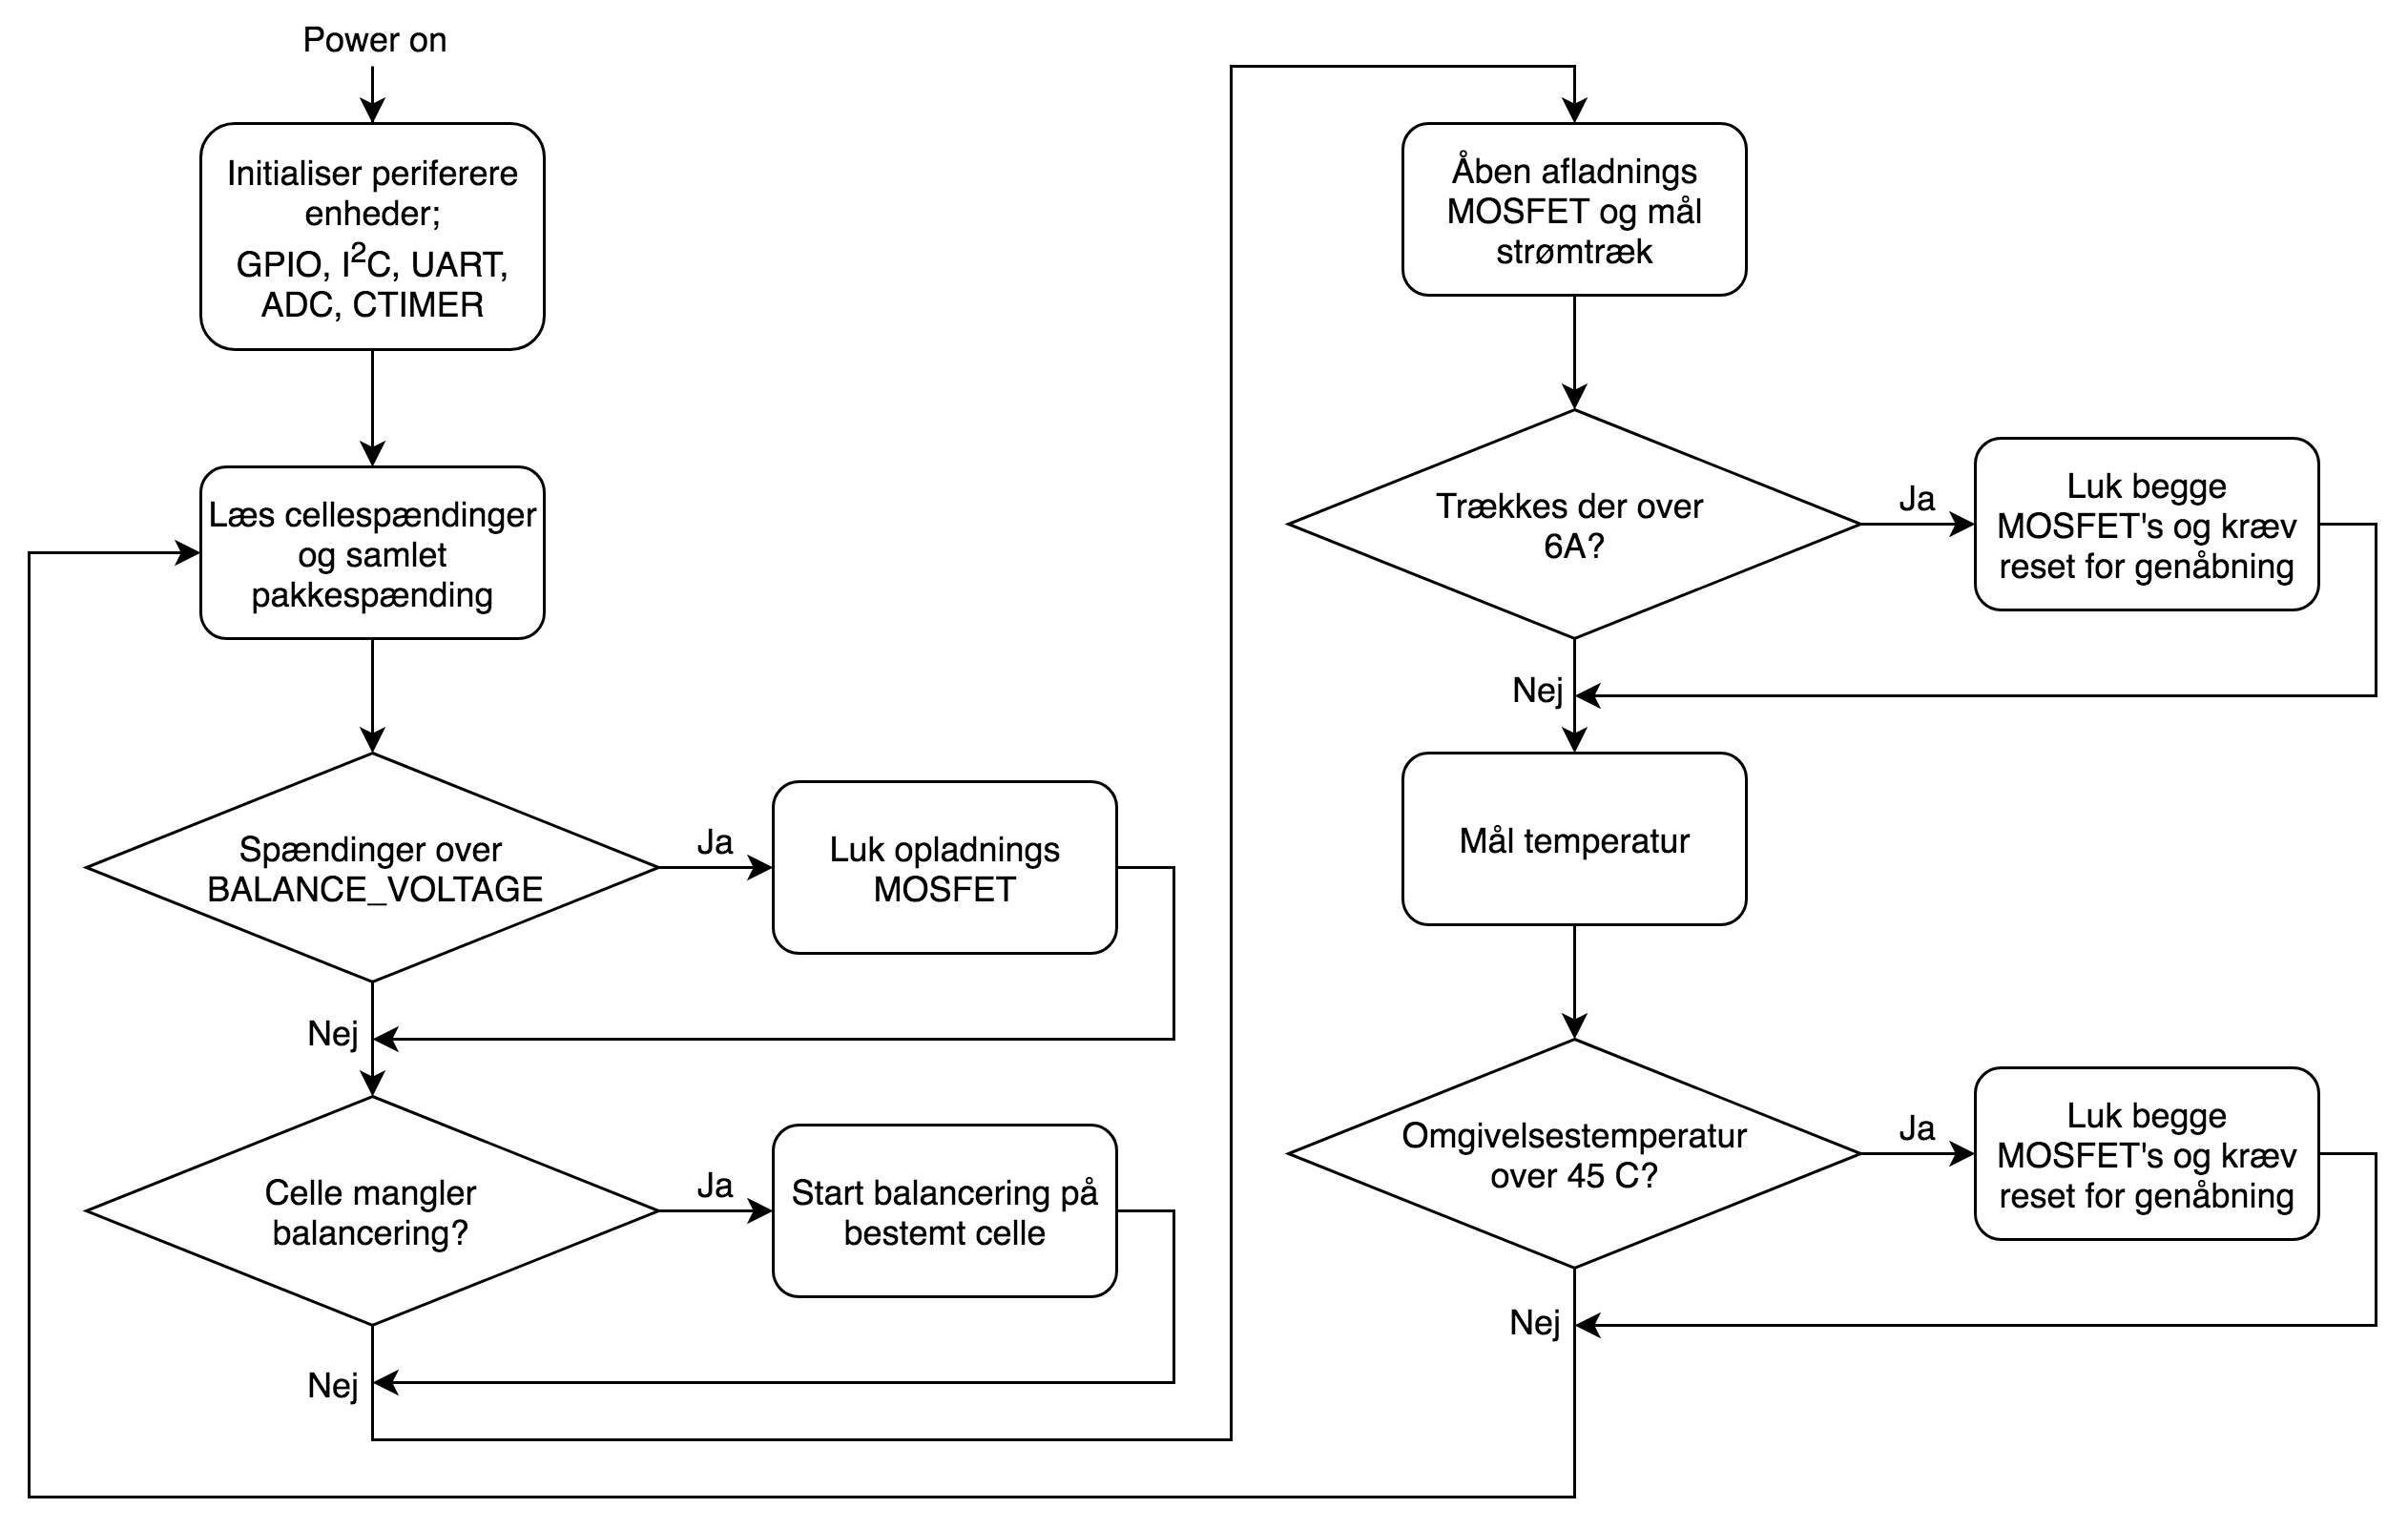
\includegraphics[width=15cm]{billeder/main_loop_bms_functions.png}
	\caption{Simplificeret flowchart over main loop (fokus på BMS funktionerne)}
	\label{fig:main_loop}
\end{figure}

Ovenstående ses flowchartet for hovedrutinen. Er

\subsection{Diskret BMS}
Den diskrete BMS bruger en del ADC'ere og GPIO pins til styring af alle funktionaliteterne, så derfor sættes disse op først. UART'en initialiseres også og en statup besked sendes. I2C initialiseres til display'et, men først til sidst da dette ikke er vigtigt for grund-funktionaliteten. \\

\subsection{Integreret BMS}
I den integrerede BMS initialiseres systemet med at klargøre alle protokoller, pins og interrupts. Som i den diskrete, sendes en startup-meddelelse til UART porten. Efter initialisation kører de fleste rutiner over I2C. BQ76920 skal initialiseres med de ønskede indstillinger i register 0x01 og 0x02. Register 0x09 skal overskrives med 0x9F under opstart ifølge databladet.\footnote{\url{http://www.ti.com/lit/ds/symlink/bq76920.pdf} side 41} \\